\section{Pairwise Loss for Pixel Embeddings}
\label{sec:max-margin}
In this section we introduce and analyze the loss we use for learning pixel
embeddings. This problem is broadly related to supervised distance metric
learning~\cite{weinberger2009distance,kong2012dictionary, kong2013learning} and clustering~\cite{kong2012multi}
but adapted to the specifics of instance labeling where
the embedding vectors are treated as labels for a variable number of objects in
each image.

Our goal is to learn a mapping from an input image to a set of $D$-dimensional
embedding vectors (one for each pixel).  Let $\x_i,\x_j \in {\mathbb R}^D$ be the
embeddings of pixels $i$ and $j$ respectively with corresponding labels $y_i$
and $y_j$ that denote ground-truth instance-level semantic labels (e.g., {\em
car.1} and {\em car.2}). We will measure the similarity of the embedding vectors
using the cosine similarity, been scaled and offset to lie in the interval
$[0,1]$ for notational convenience:
\begin{equation}
\begin{split} \small
s_{ij} = \frac{1}{2}\left(1 + \frac{\x_i^T\x_j}{\Vert\x_i\Vert_2 \Vert\x_j\Vert_2}\right)
\end{split}
\label{eq:calibrated_cosine_similarity}
\end{equation}
In the discussion that follows we think of the similarity in terms of the inner
product between the projected embedding vectors (e.g., $\frac{x_i}{\|x_i\|}$)
which live on the surface of a $(D-1)$ dimensional sphere.  Other common
similarity metrics utilize Euclidean distance with a squared exponential kernel
or sigmoid function~\cite{newell2016associative, fathi2017semantic}. We prefer
the cosine metric since it is invariant to the scale of the embedding vectors,
decoupling the loss from model design choices such as weight decay or
regularization that limit the dynamic range of Euclidean distances.

Our goal is to learn an embedding so that pixels with the same label (positive
pairs with $y_i = y_j$) have the same embedding (i.e. $s_{ij}=1$). To avoid a
trivial solution where all the embedding vectors are the same, we impose the
additional constraint that pairs from different instances (negative pairs with
$y_i \neq y_j$) are placed far apart. To provide additional flexibility, we
include a weight $w_i$ in the definition of the loss which specifies the
importance of a given pixel. The total loss over all pairs and training images
is:
\begin{equation}
\small
\begin{split}
\ell = \sum_{k=1}^M  \sum_{i,j=1}^{N_k} \frac{w^k_i w^k_j}{N_k} \Big( \1_{\{y_i=y_j\}}(1-s_{ij})
 &+ \1_{\{y_i\not=y_j\}} [s_{ij}-\alpha]_{+} \Big)
\end{split}
\label{eq:obj}
\end{equation}
where $N_k$ is the number of pixels in the $k$-th image ($M$ images in
total), and $w^k_i$ is the pixel pair weight associated with pixel
$i$ in image $k$.  The hyper-parameter $\alpha$ controls the maximum margin
for negative pairs of pixels, incurring a penalty if the embeddings for pixels
belonging to the same group have an angular separation of less than
$\cos^{-1}(\alpha)$.  Positive pairs pay a penalty if they have a similarity
less than $1$.  Fig.~\ref{fig:lossFunc} shows a graph of the loss function.
\cite{wu2017sampling} argue that the constant slope of the margin loss is more
robust, e.g., than squared loss.

\begin{figure}[t]
\vspace{-1mm}
\raisebox{-\height}{
%\vspace{-1em}
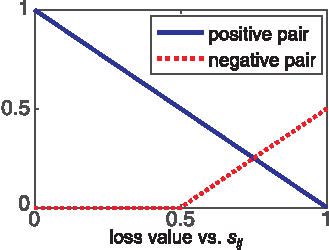
\includegraphics[width=0.20\textwidth]{proposed_lossFunc}}\hfill%
\begin{minipage}[t]{0.23\textwidth} %\vspace{-1em}%
\caption{\small
Loss as a function of calibrated similarity score Eq.~\ref{eq:calibrated_cosine_similarity}
with $\alpha=0.5$. The
gradient is constant, limiting the effect of noisy ground-truth labels
 (i.e., near an object boundary)}
\label{fig:lossFunc}
\end{minipage}
\vspace{-4mm}
\end{figure}

We carry out a simple theoretical analysis which provides a guide for setting
the weights $w_i$ and margin hyperparameter $\alpha$ in the loss function. Proofs
can be found in the appendix.

\subsection{Instance-aware Pixel Weighting}
We first examine the role of embedding dimension and instance size on the
training loss.
\begin{propositions}
\label{theorem:ObjLowerBound}
For $n$ vectors $\{\x_1, \dots, \x_n\}$, the total intra-pixel similarity is
bounded as $\sum_{i\neq j} \x_i^T\x_j \ge -\sum_{i=1}^n  \Vert \x_i \Vert_2^2$.
In particular, for $n$ vectors on the hypersphere where $\Vert\x_i\Vert_2 = 1$,
we have $\sum_{i\neq j} \x_i^T\x_j \ge -n$.
\end{propositions}
This proposition indicates that the total cosine similarity (and hence the loss)
for a set of embedding vectors has a constant lower bound that does not depend
on the dimension of the embedding space (a feature lacking in Euclidean
embeddings). In particular, this type of analysis suggests a natural choice of
pixel weighting $w_i$. Suppose a training example contains $Q$ instances and
${\cal I}_q$ denotes the set of pixels belonging to a particular ground-truth
instance $q$.  We can write
\begin{equation}
\small
\begin{split}
\| \sum_{q=1}^Q \sum_{i \in {\cal I}_q} w_i \x_i \|^2 = &
\sum_{q=1}^Q \| \sum_{i \in {\cal I}_q} w_i \x_i \|^2 + \\
&\sum_{p \neq q} \big(\sum_{i \in {\cal I}_p} w_i \x_i \big)^T \big(\sum_{j \in {\cal I}_q} w_j \x_j \big)
\end{split}
\nonumber
\end{equation}
%\begin{equation}
%\small
%\Vert \sum_{q=1}^Q \sum_{i \in {\cal I}_q} w_i \x_i \Vert^2 =
%\sum_{q=1}^Q \Vert \sum_{i \in {\cal I}_q} w_i \x_i \Vert^2 +
%\sum_{p \neq q} \left(\sum_{i \in {\cal I}_p} w_i \x_i \right)^T \left(\sum_{i \in {\cal I}_q} w_i \x_i \right)
%\nonumber
%\end{equation}
where the first term on the r.h.s. corresponds to contributions to the loss
function for positive pairs while the second corresponds to contributions
from negative pairs. Setting $w_i = \frac{1}{\vert {\cal I}_q\vert}$ for pixels $i$
belonging to ground-truth instance $q$ assures that each instance contributes
equally to the loss independent of size. Furthermore, when the embedding
dimension $D \geq Q$, we can simply embed the data so that the instance means
$ \mu_k = \frac{1}{\vert {\cal I}_q\vert} \sum_{i \in {\cal I}_q} \x_i $
are along orthogonal axes on the sphere. This zeros out the second term on
the r.h.s., leaving only the first term which is bounded
$
0 \leq \sum_{q=1}^Q \left\| \frac{1}{\vert {\cal I}_q \vert} \sum_{i \in {\cal I}_q} \x_i \right\|^2 \leq Q$,
and translates to corresponding upper and lower bounds on the loss
that are independent of the number of pixels and embedding dimension
(so long as $D \geq Q$).

%\begin{lemmas}
%\label{lemma:LowerBound4CombinationAwareWeighting}
%For $n$ embedding vectors $\{\x_1, \dots, \x_n\}$, we can choose the embedding
%loss weights so that the contribution of positive pairs is bounded by a
%constant that only depends on the number of instances since
%$\sum_q \sum_{i,j \in {\cal I}_q} \frac{1}{\vert{\cal I}_q\vert} \x_i^T\x_j \ge -Q$.
%% TODO: can we state a similar bound for negative pairs?
%%$\frac{1}{Q} \sum_{p \neq q} \sum_{i \in {\cal I}_p, j \in {\cal I}_q} \frac{1}{\vert{\cal I}_q\vert} \x_i^T\x_j \ge -1$.
%\end{lemmas}
%By setting $w_{ij} = \frac{1}{\vert {\cal I}_q \vert}$ for $i,j \in {\cal I}_q$
%we can thus balance the contribution of positive loss among instances.
Pairwise weighting schemes have been shown important empirically
\cite{fathi2017semantic} and class imbalance can have a substantial effect on
the performance of different architectures (see e.g., \cite{lin2017focal}).
While other work has advocated online bootstrapping methods for hard-pixel
mining or mini-batch selection ~\cite{loshchilov2015online, kong2016photo,
shrivastava2016training,wu2016bridging},
our approach is much simpler. Guided by
this result we simply use uniform random sampling of pixels during training,
appropriately weighted by instance size in order to estimate the loss.

\subsection{Margin Selection}
To analyze the appropriate margin, let's first consider the problem of
distributing labels for different instances as far apart as possible on a 3D
sphere, sometimes referred to as Tammes's problem, or the hard-spheres
problem~\cite{saff1997distributing}. This can be formalized as maximizing
the smallest distance among $n$ points on a sphere: $\max\limits_{\x_i\in
\RB^3} \min\limits_{i\not=j}\Vert \x_i-\x_j\Vert_2$.  Asymptotic results
in~\cite{habicht1951lagerung} provide the following proposition (see proof in the
appendix):
%\begin{propositions}
%\label{lemma:max_margin}
%Given $n$ vectors $\{\x_1, \dots, \x_n\}$ on a sphere (3D), i.e.
%$\Vert\x_i\Vert_2 = 1, \forall i=1\dots n$, then the parameter $\alpha$ in the
%maximum margin term in objective function~\ref{eq:obj} should be no less than
%$1- \Big( \frac{2\pi}{\sqrt{3}n} \Big)$ to guarantee a separation without
%inducing any loss for negative pixel pairs.  In other word, the margin
%$(1-\alpha)$ should be no larger than $\frac{2\pi}{\sqrt{3}n}$ to assure
%zero loss at an optimal separation of $n$ instances.
%\end{propositions}
\begin{propositions}
\label{lemma:max_margin}
Given $N$ vectors $\{\x_1, \dots, \x_n\}$ on a 2-sphere, i.e. $\x_i \in \RB^3$,
$\Vert\x_i\Vert_2 = 1, \forall i=1\dots n$, choosing $\alpha \leq 1- \Big(
\frac{2\pi}{\sqrt{3}N} \Big)$, guarantees that $[s_{ij}-\alpha]_{+}\geq 0$ for
some pair $i \not= j$. Choosing $\alpha > 1- \frac{1}{4} \Bigg(
\Big(\frac{8\pi}{\sqrt{3}N}\Big)^{\frac{1}{2}} -CN^{-\frac{2}{3}}\Bigg)^2$,
guarantees the existence of an embedding with $[s_{ij}-\alpha]_{+}=0$ for all
pairs $i \not= j$.
\end{propositions}
Proposition~\ref{lemma:max_margin} gives the maximum margin for a separation of $n$
groups of pixels in a three dimensional embedding space (sphere).  For example,
if an image has at most $\{4,5,6,7\}$ instances, $\alpha$ can be set as small
as $\{0.093, 0.274, 0.395, 0.482\}$, respectively.

For points in a higher dimension embedding space, it is a non-trivial problem to
establish a tight analytic bound for the margin $\alpha$. Despite its simple
description, distributing $n$ points on a $(D-1)$-dimensional hypersphere is
considered a serious mathematical challenge for which there is no general
solutions~\cite{saff1997distributing, lovisolo2001uniform}. We adopt a safe
(trivial) strategy. For $n$ instances embedded in $n/2$ dimensions one can use
value of $\alpha=0.5$ which allows for zero loss by placing a pair of groups
antipodally along each of the $n/2$ orthogonal axes. We adopt this setting for
the majority of experiments in the paper where the embedding dimension is set
to $64$.

